\subsection{Module Graph}\label{app:module-detail}

The module graph $G_{\mathrm{module}}$ (Definition~\ref{def:module-graph}; \S\ref{sec:module-import}) captures file-level import dependencies among \module{Mathlib}'s $7{,}563$ source files.

\subsubsection{Containment Decay}

Table~\ref{tab:module-containment} reports the fraction of import edges that remain within the same group at successive depths of the module tree.

\begin{table}[ht]
\centering
\caption{Module-level containment decay by module depth. At depth~$1$ ($13$ top-level packages), $97.5\%$ of import edges stay within the same package; by depth~$4$, containment has fallen to~$8.8\%$.}
\label{tab:module-containment}
\begin{tabular}{crrr}
\toprule
Depth $k$ & Groups & Containment & $\Delta$ (pp) \\
\midrule
$1$ & $13$      & $97.5\%$  & ---     \\
$2$ & $99$      & $60.2\%$  & $-37.3$ \\
$3$ & $1{,}481$ & $34.1\%$  & $-26.1$ \\
$4$ & $5{,}641$ & $8.8\%$   & $-25.3$ \\
$5$ & $7{,}434$ & $0.8\%$   & $-8.0$  \\
\bottomrule
\end{tabular}
\end{table}

At depth~$1$, the $13$ top-level packages (\module{Mathlib}, \module{Batteries}, \module{Init}, etc.) contain $97.5\%$ of all import edges. The steepest single drop occurs at depth~$1 \to 2$ ($-37.3$ pp), when packages split into their subdirectories. The $60.2\%$ containment at depth~$2$ is consistent with the $61.4\%$ intra-directory rate reported in \S\ref{sec:cross-namespace}.\footnote{The small discrepancy ($60.2\%$ vs.\ $61.4\%$) reflects a difference in edge counts between our import parser and the \texttt{importGraph} tool.} By depth~$4$ (the modal depth of modules), containment has fallen to $8.8\%$, and by depth~$5$ it is negligible.

\label{sec:structural-analysis}
\subsubsection{Degree Distribution}
\label{sec:degree-distribution}
\label{sec:sa-degree}

In $G_{\mathrm{module}}$, the out-degree $\deg^{+}(m) = |\mathrm{imports}(m)|$: it counts the number of modules that $m$ directly imports. The in-degree $\deg^{-}(m)$ counts how many other modules depend on~$m$.
Structurally, in-degree measures how foundational a module is (how many others build upon it), while out-degree measures how much of the library a module assembles. A high in-degree module is \emph{infrastructure}; a high out-degree module is an \emph{integrator}.

\begin{table}[H]
\centering
\caption{Degree statistics for $G_{\mathrm{module}}$ and its transitive reduction~$G_{\mathrm{module}}^{-}$.}
\label{tab:degree-stats}
\begin{tabular}{lrrrr}
\toprule
& \multicolumn{2}{c}{$G_{\mathrm{module}}$} & \multicolumn{2}{c}{$G_{\mathrm{module}}^{-}$} \\
\cmidrule(lr){2-3} \cmidrule(lr){4-5}
& In-degree & Out-degree & In-degree & Out-degree \\
\midrule
Mean   & $3.12$ & $3.12$ & $2.57$ & $2.57$ \\
Median & $2$    & $3$    & $1$    & $2$    \\
Std    & $4.69$ & $4.12$ & $3.91$ & $1.83$ \\
Max    & $167$  & $315$  & $151$  & $70$   \\
\bottomrule
\end{tabular}
\end{table}

The module with the highest in-degree in both graphs is \module{Mathlib.Init} ($\deg^{-} = 167$ in $G_{\mathrm{module}}$, $151$ in $G_{\mathrm{module}}^{-}$), the foundational module that most files depend on. Other high in-degree modules include \module{Tactic.Common} ($74$), \module{Analysis.Normed.Group.Basic} ($57$), and \module{Algebra.Ring.Defs} ($42$). The highest out-degree belongs to \module{Mathlib.Tactic} ($315$ in $G_{\mathrm{module}}$), which serves as an umbrella file aggregating tactic imports; transitive reduction reduces this to~$60$.

We plot the degree distributions on log--log axes (Figure~\ref{fig:degree-distribution}).

\begin{figure}[H]
\centering

\includegraphics[width=\textwidth]{figures/degree_distribution.pdf}
\caption{In-degree (blue) and out-degree (orange) distributions on log--log axes for $G_{\mathrm{module}}$ (left) and $G_{\mathrm{module}}^{-}$ (right). Dashed lines show power-law references $k^{-\gamma}$. Two features are visually salient: (i)~the in-degree distributions are nearly identical across the two panels, confirming that transitive reduction barely affects how many modules depend on a given file; (ii)~the out-degree tail contracts sharply under transitive reduction (maximum dropping from $315$ to $70$), reflecting the removal of redundant umbrella imports.}
\label{fig:degree-distribution}
\end{figure}

Both degree distributions are heavy-tailed but do not cleanly fit a power law. The out-degree distribution, in particular, becomes much more concentrated after transitive reduction (maximum dropping from $315$ to $70$, standard deviation from $4.12$ to $1.83$), indicating that many high-out-degree imports are transitively redundant.
In contrast, the in-degree distribution is barely affected by transitive reduction (maximum: $167 \to 151$; standard deviation: $4.69 \to 3.91$). This asymmetry has a structural explanation: redundant edges arise primarily from developers importing umbrella modules, an act that inflates the importer's out-degree without changing the importee's in-degree. The development-ergonomic redundancy identified in \S\ref{sec:transitive-reduction} is \emph{directional}: it lives in the ``I depend on others'' direction, not the ``others depend on me'' direction.
The redundancy is not random; it follows the contours of the module tree~$T$, because developers import umbrella modules that aggregate entire sub-hierarchies for refactoring convenience.

\subsubsection{DAG Depth}
\label{sec:dag-depth}

All sources (modules with no incoming edges) sit at level~$0$, while the unique sink \module{Tactic.Linter.DirectoryDependency} sits at level~$153$.

The depth of $G_{\mathrm{module}}$ is $153$, attained by a path from \module{NumberTheory.LSeries.PrimesInAP} (a leaf-level number theory result) down to \module{Tactic.Linter.DirectoryDependency} (a low-level linter utility). This path traverses number theory, special functions, measure theory, topology, order theory, logic, and tactic infrastructure, reflecting the deep dependency chain required to formalize analytic number theory.

$G_{\mathrm{module}}$ has $1{,}433$ source modules (files that no other \module{Mathlib} file imports) and exactly $1$~sink (\module{Tactic.Linter.DirectoryDependency}, the unique module with no imports within Mathlib). The topological levels partition $\mathcal{M}$ into $154$ layers, with a maximum layer width of $1{,}433$ (the source layer) and a median width of~$25$.

Notably, the layer-width profiles of $G_{\mathrm{module}}$ and $G_{\mathrm{module}}^{-}$ are nearly identical: the number of layers, the position of the peak, and the overall funnel shape are preserved under transitive reduction. This means that the vertical structure of the dependency chain reflects genuine logical necessity rather than cognitive redundancy; the 17.5\% redundant edges (post-\texttt{shake}) identified in \S\ref{sec:transitive-reduction} add lateral shortcuts within layers but do not alter the depth of the graph.

A secondary peak is visible near level~$126$, where approximately $59$ modules concentrate, roughly $6$ to $15$ times the width of surrounding layers. This anomaly warrants further investigation; it may reflect a layer of tactic infrastructure or a mathematical theory that branches into many parallel lemmas at a specific depth.

\begin{figure}[H]
\centering

\includegraphics[width=\textwidth]{figures/dag_structure.pdf}
\caption{DAG width by topological layer for $G_{\mathrm{module}}$ (top) and $G_{\mathrm{module}}^{-}$ (bottom). The distributions share a characteristic funnel shape: a sharp peak at level~$0$ (over $1{,}400$ leaf modules), a rapid decay through the first $20$ layers, a long tail extending to level~$153$, and a secondary peak near level~$126$. The near-identical profiles confirm that the funnel topology arises from logical necessity, not from redundant imports.}
\label{fig:dag-structure}
\end{figure}

The funnel shape (wide at the top, tapering to a single sink) reflects the fact that advanced mathematics is built on a narrow foundation of shared definitions and tactics. Any change to a module in the bottleneck layers propagates upward through a large fraction of the library, creating recompilation cascades. Lean's module system, by enabling private imports, is an existing engineering response to this narrow-waist problem.

\label{rem:import-depth-symmetry}
The DAG depth of~$153$ layers describes the topological extent of the dependency chain. A different notion of depth, the \emph{module depth} (the number of dot-separated components of a module's fully qualified name), describes how deeply a module sits in the naming hierarchy~$T$. Module depth is concentrated: $55.7\%$ of modules have depth~$4$ (e.g., \module{Mathlib.Data.Nat.Basic}), with a mean of~$4.22$. Import edges exhibit near-perfect depth symmetry: $55.4\%$ connect modules at the same naming depth, $23.3\%$ point from deeper to shallower, and $21.3\%$ from shallower to deeper (mean difference~$+0.03$). Only~$1.3\%$ of imports target modules at depth~$\le 2$. Developers import \emph{laterally}, peer to peer within the same naming stratum, rather than vertically across naming layers. As we shall see in \S\ref{sec:cross_level}, this symmetry contrasts sharply with the declaration-level dependency graph, where $37.6\%$ of edges flow from deeper to shallower namespaces and the mean depth difference rises to~$+0.36$: the module graph compresses and hides the strong infrastructure pull that the declaration graph reveals.

\subsubsection{Centrality}
\label{sec:centrality}
\label{sec:sa-centrality}

We compare three centrality measures (in-degree, PageRank, and betweenness; Definition~\ref{def:pagerank}--\ref{def:betweenness}) to identify the most structurally important modules.

\begin{table}[H]
\centering
\caption{Top~10 modules by in-degree, PageRank, and betweenness centrality in $G_{\mathrm{module}}$.}
\label{tab:centrality}
\small
\begin{tabular}{rlrlrl}
\toprule
\multicolumn{2}{c}{In-degree} & \multicolumn{2}{c}{PageRank} & \multicolumn{2}{c}{Betweenness} \\
\cmidrule(lr){1-2} \cmidrule(lr){3-4} \cmidrule(lr){5-6}
$\deg^{-}$ & Module & PR & Module & $c_B$ & Module \\
\midrule
167 & \module{Init}               & .0435 & \module{Init}              & .0113 & \module{Tactic.Common} \\
 74 & \module{Tactic.Common}      & .0316 & \module{Tactic.Linter.Header} & .0037 & \module{Init} \\
 57 & \module{AN.Group.Basic}     & .0285 & \module{Tactic.Linter.DD}  & .0032 & \module{LA.Span.Basic} \\
 45 & \module{Util.CompileInd.}   & .0058 & \module{Tactic.TypeStar}   & .0030 & \module{AN.Module.FD} \\
 42 & \module{Algebra.Ring.Defs}  & .0048 & \module{Algebra.Group.Defs} & .0024 & \module{Analysis.RCLike} \\
 39 & \module{ABO.Finset.Basic}   & .0038 & \module{Tactic.Basic}      & .0021 & \module{AS.Limits.Basic} \\
 38 & \module{Algebra.Field.Defs} & .0037 & \module{CT.Equivalence}    & .0020 & \module{AS.Limits.Normed} \\
 38 & \module{Algebra.Group.Basic}& .0033 & \module{Logic.Function}    & .0019 & \module{LA.Determinant} \\
 37 & \module{Tactic.Fin.Attr}    & .0030 & \module{Logic.Equiv.Defs}  & .0019 & \module{CT.Category.Basic} \\
 37 & \module{Tactic.TypeStar}    & .0030 & \module{CT.Opposites}      & .0017 & \module{Tactic.NormNum} \\
\bottomrule
\end{tabular}
\end{table}

\noindent
\textit{Abbreviations:} AN = \module{Analysis.Normed}, LA = \module{LinearAlgebra}, CT = \module{CategoryTheory},\\
ABO = \module{Algebra.BigOperators.Group}, AS = \module{Analysis.SpecificLimits},\\
FD = \module{FiniteDimension}, DD = \module{DirectoryDependency}, CompileInd.\ = \module{CompileInductive}, Fin.\ = \module{Finiteness}.
We compare in-degree, PageRank, and betweenness pairwise in Figures~\ref{fig:centrality-indeg-pr}--\ref{fig:centrality-betw-pr}. Out-degree is omitted from this comparison because it measures a module's role as an \emph{importer}, how many prerequisites it gathers, rather than its structural position within the network. Moreover, as shown in \S\ref{sec:degree-distribution}, high out-degree values largely reflect redundant umbrella imports and collapse under transitive reduction, making out-degree a poor proxy for structural importance.

\begin{figure}[H]
\centering
\begin{subfigure}[t]{0.32\textwidth}
\centering
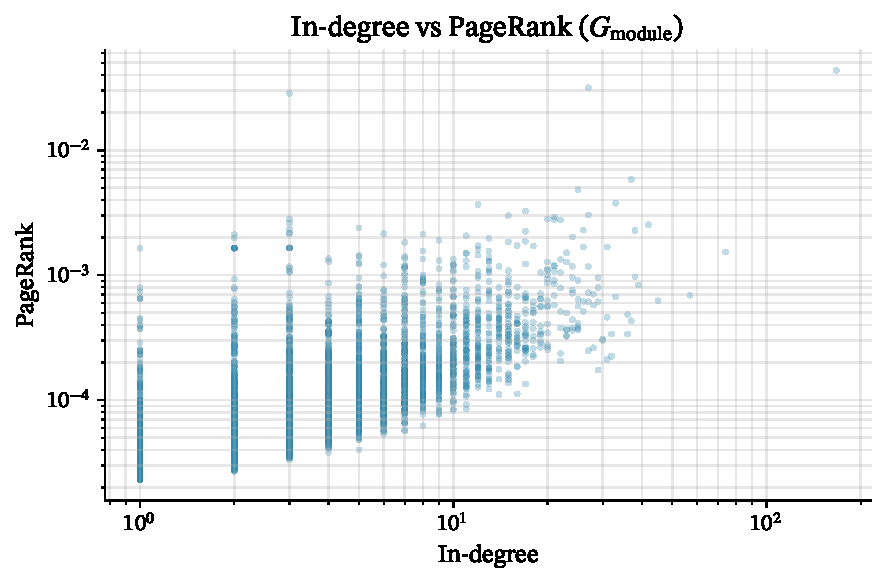
\includegraphics[width=\textwidth]{figures/module_centrality_indeg_pr.pdf}
\caption{In-degree vs.\ PageRank.}
\label{fig:centrality-indeg-pr}
\end{subfigure}%
\hfill
\begin{subfigure}[t]{0.32\textwidth}
\centering

\includegraphics[width=\textwidth]{figures/module_centrality_indeg_betw.pdf}
\caption{In-degree vs.\ Betweenness.}
\label{fig:centrality-indeg-betw}
\end{subfigure}%
\hfill
\begin{subfigure}[t]{0.32\textwidth}
\centering

\includegraphics[width=\textwidth]{figures/module_centrality_betw_pr.pdf}
\caption{Betweenness vs.\ PageRank.}
\label{fig:centrality-betw-pr}
\end{subfigure}
\caption{Pairwise centrality scatter plots for $G_{\mathrm{module}}$. Each point is one module. The wide scatter across all three panels confirms that in-degree, PageRank, and betweenness capture distinct structural roles. The three-way divergence visible in Table~\ref{tab:centrality} pervades the entire distribution, not just the top extremes.}
\label{fig:module-centrality}
\end{figure}

The three rankings largely differ: the only module appearing in all three top-20 lists is \module{Mathlib.Init}. This divergence is not a technical detail; it is one of our central findings. It demonstrates that \emph{importance} in a formal mathematical library is irreducibly multidimensional: a module can be heavily used (high in-degree) without being foundational (high PageRank), and foundational without being a bridge (high betweenness). No single centrality measure captures the full structural role of a module; the three measures together define a taxonomy that we develop further in \S\ref{sec:cross-level-summary}.

In particular, high-betweenness modules acquire their bridging role by connecting regions of $G_{\mathrm{module}}$ that the tree $T$ separates. The top betweenness modules in Table~\ref{tab:centrality} typically sit at the boundary between top-level directories, the points where mathematical logic forces a passage across $T$'s cognitive borders.

\subsubsection{Community Structure}
\label{sec:module-community}
\label{sec:sa-community}

We apply Louvain community detection (\S\ref{sec:prelim-community}) to the undirected projection of $G_{\mathrm{module}}$ ($7{,}563$ nodes, $23{,}570$ edges).

\begin{table}[ht]
\centering
\caption{Community detection summary for $G_{\mathrm{module}}$.}
\label{tab:module-community-summary}
\begin{tabular}{lr}
\toprule
Metric & Value \\
\midrule
Number of communities & $16$ \\
Modularity & $0.6395$ \\
Communities with ${>}1{,}000$ nodes & $3$ \\
Communities with ${>}100$ nodes & $9$ \\
\bottomrule
\end{tabular}
\end{table}

The modularity of $0.64$ is the highest among the three graph levels, reflecting the fact that modules are the unit at which human organization is most direct: developers place related files in the same directory, creating dense within-directory import clusters.

\begin{table}[ht]
\centering
\caption{The nine major communities of $G_{\mathrm{module}}$ (Louvain, ${>}100$ nodes), with dominant top-level directories.}
\label{tab:module-communities}
\small
\begin{tabular}{rrl}
\toprule
ID & Size & Dominant directories \\
\midrule
2  & $1{,}445$ & \module{RingTheory} (531), \module{Algebra} (377), \module{LinearAlgebra} (253) \\
7  & $1{,}398$ & \module{CategoryTheory} (893), \module{Algebra} (147), \module{Topology} (92) \\
3  & $1{,}366$ & \module{Algebra} (382), \module{Data} (297), \module{Tactic} (295) \\
1  & $948$     & \module{Analysis} (533), \module{Topology} (124), \module{Geometry} (97) \\
5  & $668$     & \module{Data} (184), \module{Order} (181), \module{Topology} (58) \\
6  & $504$     & \module{MeasureTheory} (232), \module{Probability} (112), \module{Analysis} (88) \\
4  & $455$     & \module{Topology} (233), \module{Analysis} (78), \module{Data} (41) \\
0  & $343$     & \module{Algebra} (111), \module{GroupTheory} (99), \module{Combinatorics} (52) \\
8  & $207$     & \module{Algebra} (102), \module{CategoryTheory} (38) \\
\bottomrule
\end{tabular}
\end{table}

The communities map recognizably onto mathematical domains. \module{CategoryTheory} again dominates a single community ($64\%$ of Community~$7$), mirroring the exceptional autonomy observed at the declaration level (\S\ref{sec:thm-community}). The NMI between Louvain communities and top-level directories is $0.42$ (ARI~$= 0.28$), higher than the declaration-level NMI of $0.34$ (\S\ref{sec:thm-community}). The stronger alignment reflects the fact that modules, unlike declarations, are explicitly organized into a directory tree; the import graph inherits much of that tree structure.


\subsubsection{Robustness}
\label{sec:robustness}
\label{sec:sa-robustness}

$G_{\mathrm{module}}$ is weakly connected: all $7{,}563$ modules belong to a single weakly connected component. We assess robustness by measuring the impact of targeted node removal.

\begin{table}[H]
\centering
\caption{Effect of removing the top-5 modules (by in-degree or betweenness) on the number of weakly connected components.}
\label{tab:robustness}
\begin{tabular}{lrr}
\toprule
Removal strategy & \multicolumn{1}{c}{$G_{\mathrm{module}}$} & \multicolumn{1}{c}{$G_{\mathrm{module}}^{-}$} \\
\midrule
None (baseline)          & $1$  & $1$  \\
Top-5 by in-degree       & $29$ & $56$ \\
Top-5 by betweenness     & $20$ & $48$ \\
\bottomrule
\end{tabular}
\end{table}

Removing the five highest in-degree modules (\module{Init}, \module{Tactic.Common}, \module{Analysis.Normed.Group.Basic}, \module{Util.CompileInductive}, and \module{Algebra.Ring.Defs}) fragments the raw graph into $29$ components, though the largest component still contains $7{,}530$ of the original $7{,}563$ nodes. The effect is more pronounced on $G_{\mathrm{module}}^{-}$ ($56$ components), since transitive reduction removes the alternative paths that would otherwise keep the graph connected.

\label{rem:robustness}
Even after targeted removal, over $99\%$ of modules remain in the giant component. The transitive reduction is more fragile ($56$ components vs.\ $29$) precisely because it removes the redundant connectivity that doubles as structural insurance.

\begin{figure}[ht]
\centering

\includegraphics[width=\textwidth]{figures/module_robustness_curve.pdf}
\caption{Robustness curves for $G_{\mathrm{module}}$: fraction of nodes in the largest WCC as a function of the fraction removed, under random removal (blue) and targeted removal by PageRank (coral).}
\label{fig:module-robustness}
\end{figure}

Figure~\ref{fig:module-robustness} shows the progressive removal curves. Under random removal, the giant component degrades gracefully: removing $20\%$ of modules leaves $80\%$ connected. Under targeted attack on the highest-PageRank modules, the same $20\%$ removal reduces the giant component to $58\%$, a $22$-percentage-point gap that grows with the removal fraction. The curve confirms the hub-dominated vulnerability signature: the module graph's resilience depends on a small number of high-centrality hubs whose removal fragments the network far more effectively than chance would predict.

\subsubsection{Extended Analysis}\label{app:module-analysis}

The $17.5\%$ post-\texttt{shake} edge redundancy (\S\ref{sec:transitive-reduction}) represents a \textit{development ergonomics layer}: developers import umbrella modules to bring tactics, notation, and typeclass instances into scope, sacrificing logical minimality for usability. The fact that \texttt{shake} intentionally preserves many of these imports confirms they serve a structural purpose, suggesting that future proof assistants could benefit from explicitly modeling two dependency layers: a minimal graph for the build system and a richer graph for the interactive environment.

The layer-width profile (\S\ref{sec:dag-depth}) reveals a \textit{funnel topology}: a massive leaf layer (${>}1{,}400$ modules) resting on a deep, narrow foundation. Changes in the narrow ``waist'' (high-betweenness modules) trigger recompilation cascades, a scalability challenge that Lean's module system (November 2025) addresses through private imports. Unlike informal mathematics, where foundational texts are static, \module{Mathlib}'s foundational modules remain mutable code; the maintenance cost of a module is a function of its topological depth. One possible trajectory is that monolithic libraries will hit a \textit{critical depth threshold} requiring \textit{federated tiers}, freezing foundational layers into pre-compiled artifacts.

The three centrality measures (\S\ref{sec:centrality}) admit distinct operational interpretations: in-degree identifies frequently used \textit{vocabulary}; PageRank identifies the \textit{axiomatic core}; betweenness identifies \textit{structural bridges} between subfields. Refactoring a high-betweenness module carries more systemic risk than refactoring a high-in-degree module, since it disrupts cross-theory connectivity.

We hypothesize that \module{Mathlib} has evolved into a \textit{curated small-world network}, growing via \textit{semantic attachment} rather than preferential attachment: new modules cluster within directories while bridge modules maintain global connectivity. The module tree~$T$ and the import graph~$G_{\mathrm{module}}$ continuously reshape each other: developers import along cognitive contours of~$T$, while cross-directory dependencies force periodic reorganization, as in the ongoing absorption of \module{RingTheory} into \module{Algebra}.
